\documentclass[a4paper, 12pt]{article}

%\usepackage{savetrees}
\usepackage{graphicx}

%code for creating python code snippets
\usepackage{float}
\floatstyle{ruled}
\newfloat{python}{thp}{lop}
\floatname{python}{Listing}
%end code for creating python code snippets

\graphicspath{{./images/}}
\title {Student Robotics 2009\\ Power Board Documentation}
\date{\today}
\setcounter{tocdepth}{1}


\begin{document}

\maketitle

\noindent This document describes the functions of the Power Board. 

\begin{figure}
\centering
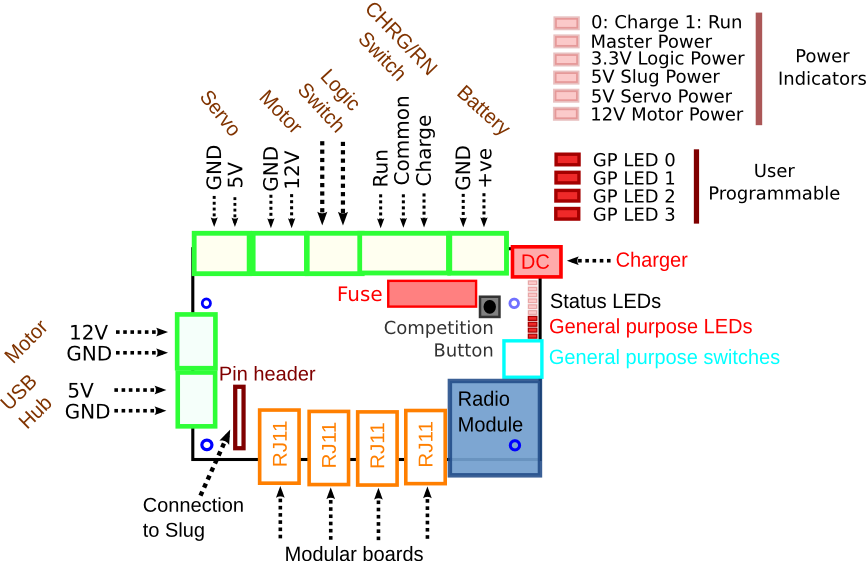
\includegraphics[scale=1, angle=90]{outline}
\caption{Power Board 1:1 Scale Drawing}
\label{fig:outline}
\end{figure}


\section{Board Outline}
Figure \label{fig:outline} is a 1:1 scale drawing of the power board which can be printed out and used to aid drilling holes for mounting.
\label{sec:outline}

\section{Brief Description}
The power board generates the power supplies necessary for the motors and control electronics. In addition it provides data connections to all of the Student Robotics boards, via the black, RJ11 Cables. During the competition, the Power Board also houses a radio module which allows your team's robot to be sent the \textit{go} and \textit{stop} commands at the beginning and end of competition rounds.

For instructions on how to assemble the power board and Student Robotics kit, see \textit{Student Robotics Assembly Guide 2009}, available from the website.

\section{Powering your Robot, Charge vs. Run Mode}
There are two ways of powering your robot:
\begin{enumerate}
\item 12V Sealed Lead Acid Battery (supplied)
\item 12V Mains regulated battery charger (supplied)
\end{enumerate}

These correspond to two distinct modes of operation: \textbf{charge mode} \& \textbf{run mode}. In \textbf{charge mode}, if the battery charger is plugged in, your robot's battery will charge. You can continue to operate your robot whilst in this mode however, the motors will be \textbf{deactivated} (this is to stop the robot running away from the mains socket). 

\vspace{12pt}
In \textbf{run mode} the motors will be activated and your robot will be fully functional. It should be noted that in this mode the battery \textbf{will not charge} even if the charger is connected! It is \textbf{required} that you mark clearly the two modes next to, or on, the switch.

\section{Competition Button}
When you turn your robot on, the slug will boot and then wait until it receives the \textit{go code} over its radio module before executing your code. During testing it will never receive this signal, so you must press the competition button on the power board to override this feature. If you do not, the slug will wait indefinitely for either the radio signal or the button push. 

\vspace{12pt}

Pressing the competition mode button before the slug has booted may not work. It is recommended that you wait until the slug has booted before pressing the button. 

\section{Radio Module}
You will be supplied with the radio module on the day of the competition. It is not required during testing \& developing.

\section{Additional Motors and Electronics}

In addition to the supplied Student Robotics Kit, you can add additional motors and electronics to your robot. To aid with this, there is a spare 12V power connector provided on the Power Board through which \textbf{all additional electronics must be powered}. Devices connected in this way are subject to the same restrictions as the Motor Board, i.e.\ they are only powered when in Run mode.

\vspace{12pt}

Spare connectors are supplied in your kit for this purpose.


\section{General Purpose Switches}

In addition to the IO features of the JointIO board, the Power Board has a bank of four DIP switches which can be read by your python code. These may be used to select between strategies depending on the current game type (Golf or Squirrel). Additionally, they may be used during testing to switch between different test routines. 

\begin{python}
\begin{verbatim}

	bee = sw(0)		%insert proper code here 

\end{verbatim}
  \caption{Reading the Power Board general purpose Switches in Python} 
\end{python}

\section{General Purpose LEDs}
Four general purpose LEDs are provided on the power board to be used when debugging your code. They can be set from within your python code and may be configured to flash when a block is detected by the vision system, or when a particular block of code is being executed.

\begin{python}
\begin{verbatim}

	setleds(0) = 1		%insert proper code here 

\end{verbatim}
  \caption{Setting the Power Board general purpose LEDs in Python} 
\end{python}

\section{Trouble shooting}
\subsection{No lights illuminate}
Is the fuse fitted and not blown? Is the battery or charger connected? Is the battery charged?

\subsection{The Slug never boots/beeps}
Are both memory sticks plugged in to the USB Hub? Is the USB Hub powered? Is the battery flat? Is the slug connected to the power board correctly? 

\subsection{Our code never runs}
Have you pressed the competition button to override waiting for the radio signal? Have you checked the syntax of your code using the IDE?

\subsection{The lights on the motor board flash, but the wheels don't turn}
Are you in Run mode? Have you wired up the connector correctly?
\end {document}
